\section{La Qualité}

	%						%
	%  PREMIERE PARTIE		%
	%						%

\subsection{Développement et tests}

% Première slide %
\begin{frame}
  \frametitle{\color{white} Développement et tests}
  \begin{center}
    \begin{tikzpicture}[scale=1]
      \umlbasicstate[x=0, name=task1, width=8ex]{Tâche 1}
      \umlbasicstate[x=3, name=task2, width=8ex]{Tâche 2}
      \umlbasicstate[x=6, name=task3, width=8ex]{Tâche 3}
      \umlbasicstate[x=0, y=-2.5, name=dev1, width=6ex, fill=green!20]{Dev Princ}
      \umltrans{dev1}{task1}
      \umlbasicstate[x=3, y=-2.5, name=dev2, width=6ex, fill=green!20]{Dev Princ}
      \umltrans{dev2}{task2}
      \umlbasicstate[x=6, y=-2.5, name=dev3, width=6ex, fill=green!20]{Dev Princ}
      \umltrans{dev3}{task3}
      \umlbasicstate[x=1.5, y=-5, name=sup1, width=7ex, fill=red!20]{Dev Support}
      \umltrans{sup1}{dev1}
      \umltrans{sup1}{dev2}
      \umlbasicstate[x=4.5, y=-5, name=sup2, width=7ex, fill=red!20]{Dev Support}
      \umltrans{sup2}{dev2}
      \umltrans{sup2}{dev3}
    \end{tikzpicture}
  \end{center}
\end{frame}

% Deuxième slide %
\begin{frame}
  \frametitle{\color{white} Types de tests}
  \begin{itemize}
  \item Tests unitaires
  \item Tests d'intégration
  \item Tests de non-régression
  \item Tests d'acceptation
  \end{itemize}
  
  
\end{frame}


	%						%
	%  SECONDE PARTIE		%
	%						%

\subsection{Stratégie de test}
% Troisième slide %
\begin{frame}
  \frametitle{\color{white} Stratégies de test}
  \begin{block}{Approche choisie pour les tests}
   Ecriture des tests automatisés puis écriture du code pour faire passer le test
  \end{block}
  \begin{figure}[p]
    \centering
    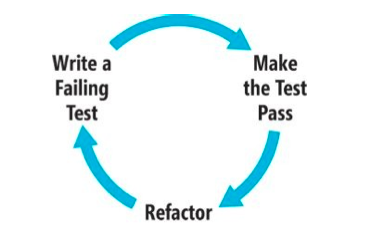
\includegraphics[scale=.25]{tests.png}
    \caption{Développement dirigé par les tests}
  \end{figure}
\end{frame}


	%						%
	%  TROISIEME PARTIE		%
	%						%

\subsection{Risque}
% Quatrième slide %
\begin{frame}
  \frametitle{\color{white} Risque qualité}
  Que faire dans le cas de la perte d'un membre ?

\end{frame}


